%----------------------------------------------------------------------------------------
%	GUISDAP.
%----------------------------------------------------------------------------------------

\section{GUISDAP software}
In this section the raw EISCAT data is processed using the MATLAB software with the package GUISDAP. The data analyzed in this section was obtained with the 42m radar located in Svalbard, Norway. The time frame of the analyzed data corresponds to the 27th of October, 2016, from 15:00 to 21:00.
\newline
\newline
GUISDAP have several "experiment" methods. From the EISCAT experiments manual: "An EISCAT experiment is a set of instructions telling the transmitters, receivers and digital signal processing units what to do at what time". Meaning that depending on the object of interest of the experimenter, Some of the parameters that change between experiments are the code length in bits, baud length, smapling rate, the range span (measurable height), time resolution, etc. In this particular case, the experiment "ipy" was used. 
%\begin{tabular}[H]{c | c}
%	Version & 4.2 \\\hline
%	Antenna & Single, switchable\\\hline
%	
%\end{tabular}
\newline
\newline
With the help of GUISDAP, a few plots showing different parameters observed in the ionosphere at the time period mentioned above. The following parameters are used by the ipy experiment. One of the obtained parameters is the raw electron data. The data obtained with GUISDAP which is data measured from the EISCAT radar, was compared with data formulated using the IRI model in the following pictures.

\begin{minipage}{0.45\textwidth}	
	\begin{flushleft}
	\begin{figure}[H]
		\centering
		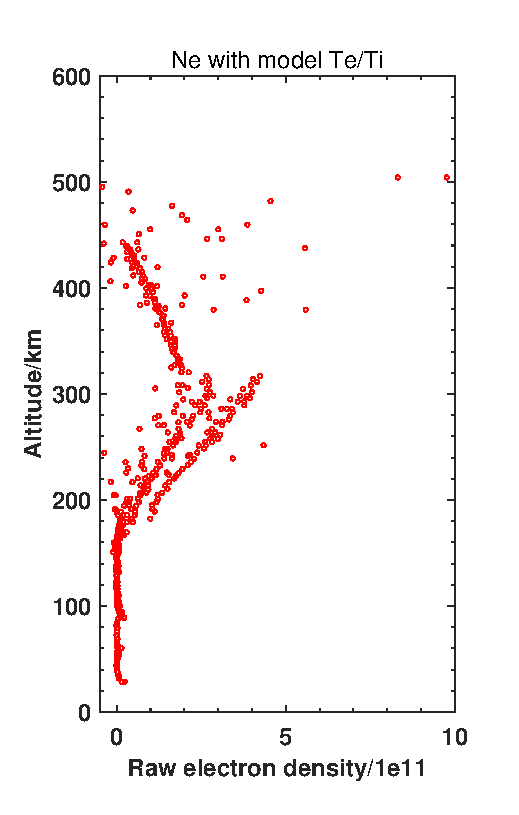
\includegraphics[width=\textwidth]{figures/rawNe.eps}
		\caption{Electron density data obtained from EISCAT 2016-10-27.}
		\label{fig::NeE}
	\end{figure}
	\end{flushleft}
\end{minipage}
\begin{minipage}{0.45\textwidth}
	\begin{flushright}
	\begin{figure}[H]
	\centering
	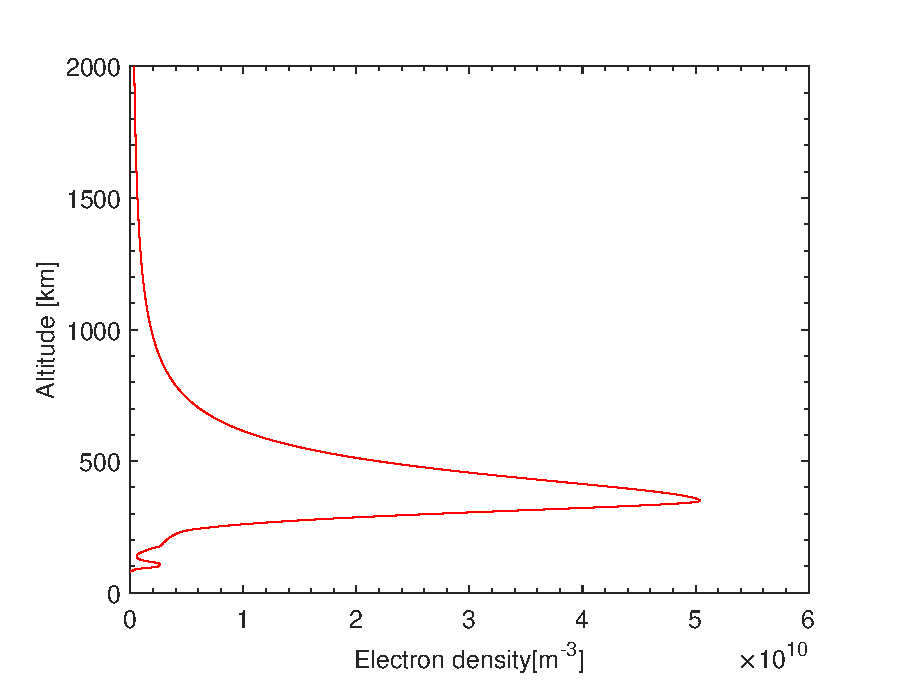
\includegraphics[width=\textwidth]{figures/NeIRI.eps}
	\caption{Electron density data from the IRI model 2016-10-27}
	\label{fig::NeIRI1}
	\end{figure}
	\end{flushright}
\end{minipage}

In these two images, the electron density from 0 to 600 km was plotted in order to compare the IRI model to the measurements from EISCAT. Both are showing the electron density distribution at around 18:00 hours. While both the model and measurements agree on where the maximum occurs, the model underestimates the amount of electrons by about a factor of 3. This discrepancies can be attributed to any assumptions that the model might take.

\begin{figure}[H]
	\centering
	\includegraphics[width=0.90\textwidth]{figures/Results.eps}
	\caption{Plot produced analyzing raw data from EISCAT with GUISDAP}
	\label{fig::resultsE1}
\end{figure}

Figure \ref{fig::resultsE1} shows the results of analyzing 6 hours of data obtained by EISCAT from 15:00  to 21:00 on the 27th of October 2016. In the first row, we can see the electron density which matches with the plots on figure \ref{fig::NeE} and figure \ref{fig::NeIRI1}, showing a maximum around 300 km of altitude. The second row shows the electron temperature, with respect to each altitude, it is interesting to note that most of the times the variation is smooth and small, except for a small band right before 18:00 and a larger band around 20:30. The third row row shows the ion temperature, again, this one is more or less constant along time with a few exceptions around 17:30 and 18:00. The fourth row showing the ion drift velocity,  most of the values look like a more or less random noise, meaning that this drift velocity is not consistent. On the fifth and final row we see the data of the antenna  within the time range of the data analyzed.